\chapter{Introduction}
\label{c:intro}

\section{Motivation}
\label{s:motivation}

%
% Why we need an online analysis platform
%

As more and more genome-wide studies rely on next-generation sequencing (NGS)
analysis, there is an increasing demand from both researchers and clinicians to
develop systems to orchestrate and interpret NGS data analysis pipelines. NGS
provides high read throughput which can generate total a few giga base pairs of
read sequences in a typical experiment run. However, before the read sequences
yielding biologically meaningful results, they have to undergo many non-trivial
steps including genome alignment, sequence piling up, variant calling, and
transcript expression quantification which requires hours of computation by
high-end processors.

Combining the demand for fast computation speed and large data storage, NGS
analyses are mostly performed on powerful servers remotely using command line
interface. Therefore, the tools involved are often developed without graphical
interface due to maximum computation efficiency and lack of need. This kind of
terminal-based environment imposes a high barrier for especially biologists and
clinicians to enter. Furthermore, output of most analysis tools are shown as
log files or as file formats that are friendly for computers to parse but can
not be easily interpreted by human without data cleaning and transformation.

As a NGS service core lab, many lab members have identified the burden of
routine NGS data processing and interpretation of results of commonly used
analysis pipelines. If a graphical summary report can be obtained after the
automated execution of analysis pipeline, many biologists and clinicians can
interpret the result themselves without extensive knowledge of how computers
work nor consulting bioinformatic researchers and thus improve the efficiency
of collaboration. On the other hand, for bioinformatic researchers, automated
execution of typical analysis pipelines can release them from routine tasks to
process incoming NGS experiment runs and focus more on innovative discovery and
interpretation of the NGS data itself.

Several analysis platforms have been proposed to help automate NGS analysis
pipeline with user friendly report or result viewer, including commercial
products such as DNAnexues \cite{:dnanexus} and Partek Flow \cite{:partek} and
open source projects such as Galaxy \cite{goecks2010:galaxy} and Genome
Modeling Tools \cite{griffith2015:genome}. However, these tools are either too
complex for biological researchers and clinicians to use, too simple for
researchers to build their own pipeline, or operating at a scale too large for
our lab to adapt. Therefore, the idea of building our own designed NGS online
analysis platform then emerged and became the main goal of my master thesis
study.


\section{Specific Aims}
\label{s:specific-aim}

%
% Propose the analysis platform and report generator
%

\section{Next-generation sequencing}
\label{s:ngs}

Next-generation sequencing is a group of sequencing technologies that succeeds
automated Sanger sequencing by providing much higher read throughput while
shorter read length that reduces the cost and time to complete genome-wide
sequencing study \cite{metzker2010:sequencing}. In the last decade,
next-generation sequencing has become the \textit{de facto} way to understand
genome \cite{vandijk2014:ten} including quantification of transcriptome
expression \cite{wang2009:rnaseq}, variant calling and genotype inference
\cite{nielsen2011:genotype}.


Next-generation sequencing has been playing an important role in current genomic
researches in the last decade.

% Sanger - 1st gen
% next-generation - 2nd gen

\section{RNA sequencing application}
\label{s:rna-seq-app}

\section{DNA sequencing application}
\label{s:dna-seq-app}

\section{Genome reference}
\label{s:genome-ref}



% Recently a cat appears in NTU as shown in Figure~\ref{i:cat}.
% This is English line spacing test. You should see double spacing text.
% This is English line spacing test. You should see double spacing text.
% This is English line spacing test. You should see double spacing text.

%i:cat
\begin{figure}[!htbp]
\centering
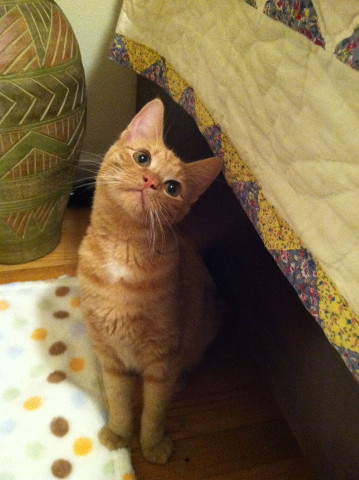
\includegraphics[width=0.58\textwidth]{images/cat}
\caption{A cat.}
\label{i:cat}
\end{figure}


% vim: set tw=79:
